Las proteínas son macromoléculas formadas por cadenas lineales de
aminoácidos, cada una de las cuales se denomina polipéptido. El
término \textbf{proteína} se origina del griego \textit{proteios} que
significa ``primario'' o ``de primer orden''. El nombre fue adoptado
por Jöns Berzelius en 1838 para enfatizar la importancia de esta clase
de moléculas. Las proteínas juegan un rol crucial en el mantenimiento
de la vida, ya que son el soporte para la arquitectura del tejido
muscular, ligamentos, tendones, huesos, piel, cabello, órganos y
glándulas. Proveen los servicios fundamentales de transporte y
almacenamiento como en el caso del oxígeno y hierro en células
musculares y eritrocitos. También participan en muchos procesos
regulatorios esenciales, como reacciones de catálisis, funciones
inmunológicas y hormonales, así como en la coordinación de actividades
neuronales y diferenciación celular.\cite{tamar}

\begin{figure}[H]
  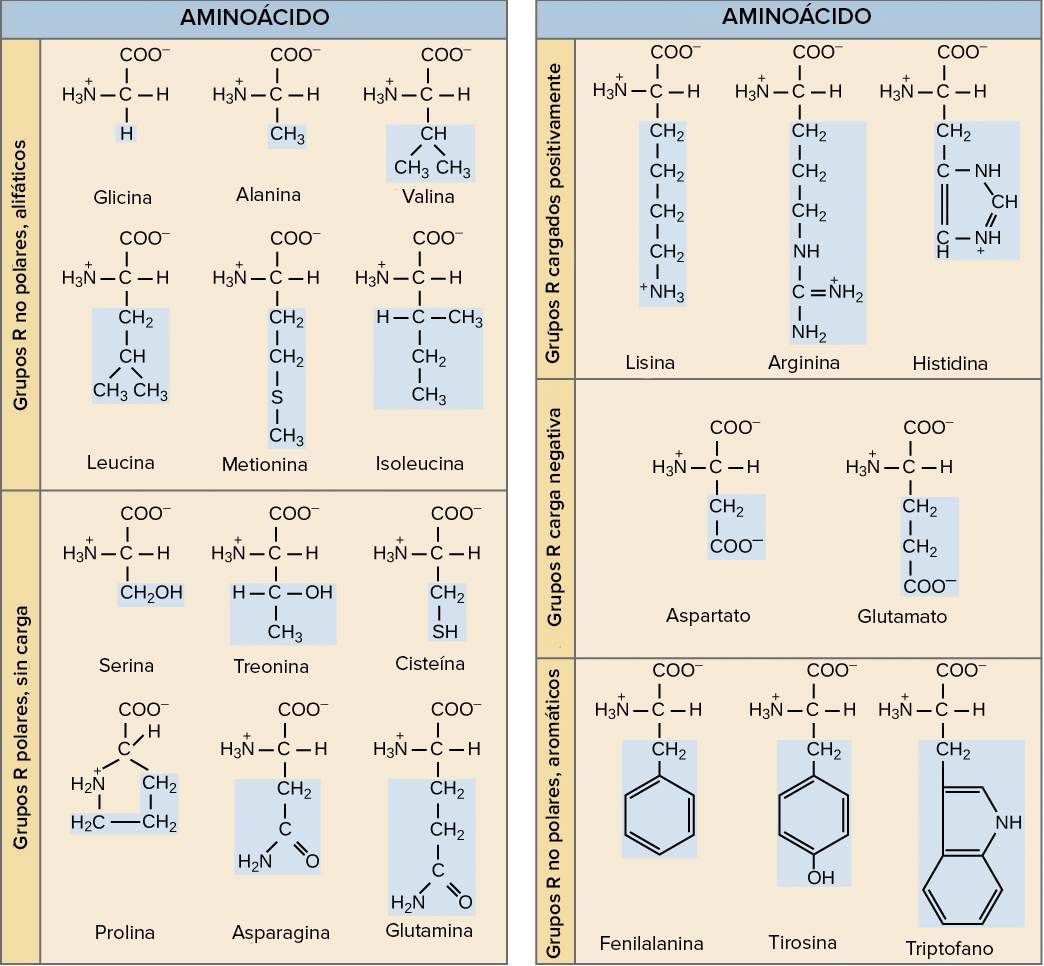
\includegraphics[scale=0.3]{aminoacids} \centering
  \caption{Existen sólo 20 tipos de aminoácidos en las proteínas
  (Tomado de \url{https://cnx.org/contents/GFy_h8cu@11.9:2zzm1QG9})}
\end{figure}

\section{Ligandos}
La comunicación entre moléculas es dada por medio de señales químicas.
Estas señales químicas son mandadas en forma de moléculas pequeñas,
usualmente volátiles o solubles, llamadas ligandos.
Un \textbf{ligando} es una molécula que se une a otra molécula
específica, en algunos casos, mandando una señal en el proceso. Los
ligandos interactuan con proteínas en células objetivos.  Son a estas
proteínas a las que llamamos \textbf{receptores}.

Las interacciones de una proteína con otras moléculas, como ligandos,
ácidos nucléicos u otras proteínas, son críticas para su función
bioquímica. Usualmente, no todos los residuos en la superficie de una
proteína participan en estas interacciones; las interacciones ocurren
en áreas definidas, que llamamos \textbf{sitios de activación o
activos} de las proteínas.

Las interacciones proteína-ligando y proteína-proteína juegan un papel
fundamental en el descubrimiento de fármacos: el objetivo de la
creación de fármacos es encontrar un agente que pueda interactuar con
una molécula objetivo y modificar su actividad. Estas moléculas
objetivo son usualmente proteínas, encargadas de la mayoría de las
tareas necesarias para mantener a las células vivas. Por otro lado,
los agentes son ligandos que interactuan con el sitio activo de la
proteína y pueden inhibirla o reactivarla, de ahí que a este tipo de
ligandos se le llamen \textbf{inhibidores}. Es por esto que se han
desarrollado una variedad de metodologías para investigar dichas
interacciones. En este trabajo nos enfocamos en el acoplamiento
molecular.

\section{Acoplamiento molecular}
El campo del \textbf{acoplamiento molecular} o
\textbf{docking} surge a lo largo de las últimas tres décadas gracias a la
necesidad de la biología molecular en cuanto al descubrimiento de
inhibidores basado en estructuras. Este campo ha evolucionado
considerablemente a lo largo de los últimos años gracias al
crecimiento dramático en la disponibilidad y poder de las
computadoras, además del incremento en las bases de datos de proteínas
y moléculas, y la facilidad de acceso a ellas.\cite{kukol}

\begin{figure}[H]
  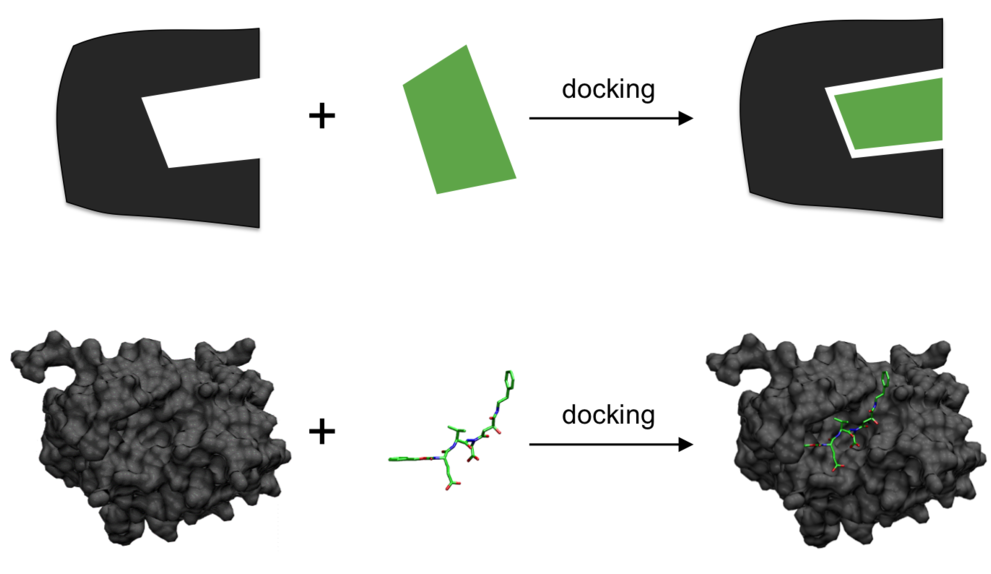
\includegraphics[scale=0.3]{docking} \centering
  \caption{Representación esquemática del \textit{docking}.  (Tomado de
    \url{https://en.wikipedia.org/wiki/Docking_(molecular)})}
\end{figure}

El objetivo de un programa de acoplamiento molecular automatizado es
comprender y predecir reconocimiento molecular, tanto
estructuralmente, encontrando posibles \textit{poses} de acoplamiento,
como energéticamente, prediciendo la afinidad del enlace. El
acoplamiento molecular usualmente se realiza entre una molécula
pequeña, un ligando, y una macromolécula objetivo, una proteína en
nuestro caso. Es importante que este acoplamiento se haga en el sitio
activo del receptor, ya que es ahí donde se espera que se dé la
interacción.

\begin{center}
\begin{figure}[H]
  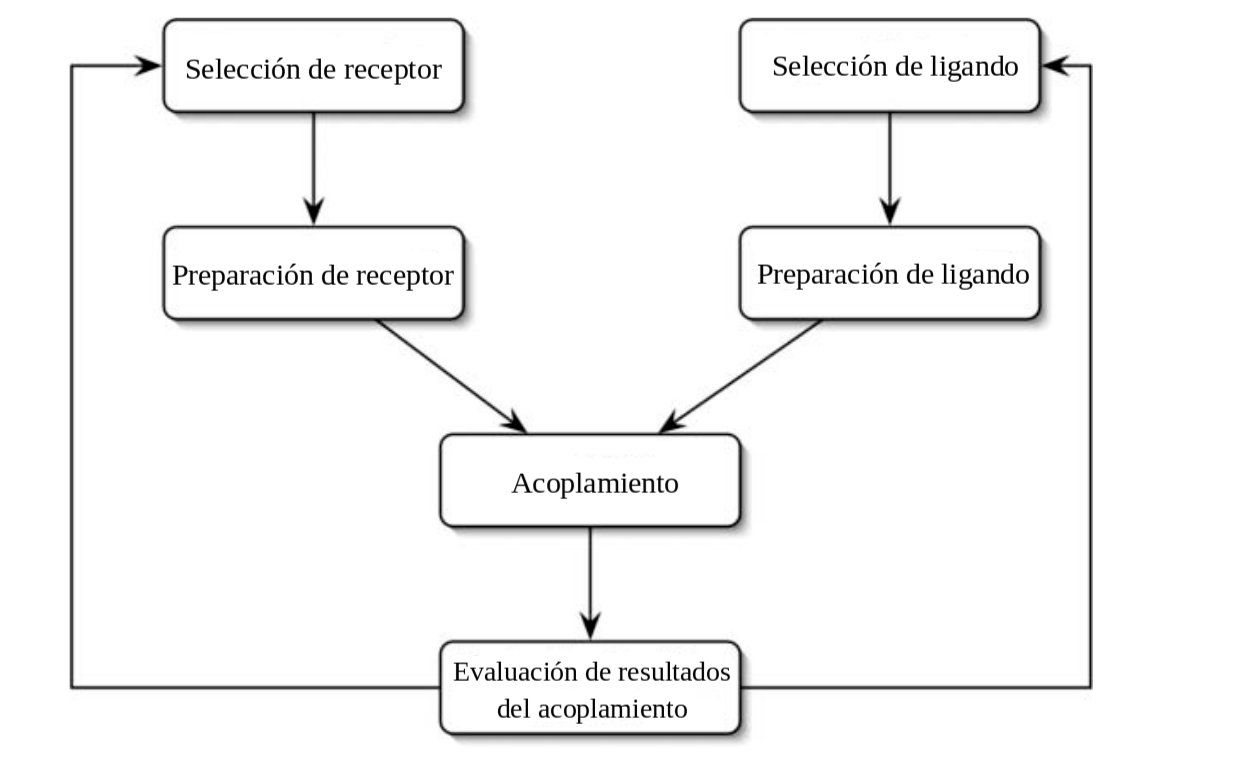
\includegraphics[scale=0.3]{docking_steps}
  \caption{Diagrama de flujo para un acoplamiento usual.  (Tomado de
    \cite{kukol})}
  \label{fig:docking_flowchart}
\end{figure}
\end{center}

La figura \ref{fig:docking_flowchart} muestra los pasos clave que son
comunes en todos los protocolos. El acoplamiento consiste en encontrar
las poses de unión más favorables de un ligando hacia una proteína
objetivo. La pose de unión de un ligando puede ser caracterizado de
forma única por sus variables de estado. Éstas consisten en su
posición (traslaciones sobre los ejes $x, y, z$), orientación (ángulos
de Euler o cuaterniones) y, si el ligando es flexible, su conformación
(los ángulos de torsión para cada enlace de rotación). Cada una de las
variables de estado describe un grado de libertad en un espacio de
búsqueda multidimensional.

\section{Función evaluadora}
Todos los métodos de acoplamiento requieren una función de evaluación
para calificar las poses de unión de los candidatos, y un método de
búsqueda para explorar las configuraciones de las variables de
estado. En general, el éxito de un acoplamiento se mide en términos de
la \textbf{desviación media cuadrática}
(RMSD, \textit{Root-mean-square deviation}) de las coordenadas
cartesianas de los átomos del ligando en las conformaciones del
acoplamiento, comparadas con las cristalográficas. Un acoplamiento se
considera exitoso si el RMSD es menor a 2\AA.\@
